%---------- Inleiding ---------------------------------------------------------

\section{Introductie}%
\label{sec:introductie}

% Met een jaarlijks budget van 32 miljoen in het vakgebied kunstmatige intelligentie (AI) op de werkvloer is België een pionier \autocite{Crevits2022}.  Zo zijn er verschillende projecten, om taalgerelateerde AI-ontwikkelingen op te starten, uit de grond gestampt. Het amai!-project \footnote{https://amai.vlaanderen/}  verenigt AI-softwarebedrijven uit verschillende domeinen om zo met AI-toepassingen te maken die processen automatiseren om de werkdruk te verminderen, zoals binnen het onderwijs \textit{real-time} ondertiteling en een taalassistent voor leerkrachten in meertalige klasgroepen.

Het Vlaamse middelbaar onderwijs staat nu op barsten, aangezien leraren en scholieren worden overspoeld door werkdruk en stress. Bovendien is de derde graad van het middelbaar onderwijs een belangrijke mijlpaal voor de verdere loopbaan van scholieren, hoewel deze het moeilijk hebben om grip te krijgen op de vakliteratuur binnen STEM-vakken \autocite{Dapaah2022}. Het STEM-agenda\footnote{https://www.vlaanderen.be/publicaties/stem-agenda-2030-stem-competenties-voor-een-toekomst-en-missiegericht-beleid} van de Vlaamse Overheid bestaat uit aandachtspunten om het STEM-onderwijs tegen 2030 aantrekkelijker te maken, door de ondersteuning voor zowel leerkrachten als scholieren te verbeteren. Toch wordt het aanpakken van de steeds complexere wetenschappelijke taal, zoals beschreven in \textcite{Barnett2020}, niet als prioriteit beschouwd binnen de STEM-agenda. Het vereenvoudigen van wetenschappelijke artikelen, op maat van de verschillende noden voor een scholier met dyslexie in het middelbaar onderwijs, is tijd- en energie-intensief. Geautomatiseerde en adaptieve tekstvereenvoudiging biedt hier een baanbrekende oplossing om de werkdruk te verminderen.

Het doel van dit onderzoek is om uit te wijzen  een toepassing moet hebben om adaptieve en geautomatiseerde tekstvereenvoudiging aan te bieden aan scholieren met dyslexie in het middelbaar onderwijs. De volgende onderzoeksvraag wordt opgesteld: "Hoe kan de inhoud van een wetenschappelijke artikel op een geautomatiseerde wijze vereenvoudigd worden, specifiek gericht op de verschillende behoeften van scholieren met dyslexie in de derde graad middelbaar onderwijs?" 

Er wordt gestart met een theoretische basis voor tekstvereenvoudiging en een literatuurstudie naar welke uitdagingen een dergelijke toepassing in acht moet nemen. In een vervolgstap wordt met een veldonderzoek gekeken naar bestaande AI toepassingen voor tekstvereenvoudiging in Nederlandstalige en Engelstalige teksten. Hierna beschrijft het onderzoek een pipeline voor geautomatiseerde tekstvereenvoudiging en staat het stil bij de verschillende metrieken om een vereenvoudigde tekst te beoordelen. Daarna vindt een vergelijkende studie. De resultaten van het onderzoek worden gebruikt om inzicht te krijgen in hoe wetenschappelijke artikelen op een geautomatiseerde en adaptieve manier vereenvoudigd kunnen worden, specifiek voor scholieren met dyslexie in het derde graad middelbaar onderwijs. Dit leidt tot verdere ontwikkeling voor AI-ontwikkelaars om een bruikbare toepassing te creëren voor gebruik in het onderwijs.

Hoofdstuk 2 biedt een overzicht van de literatuur over geautomatiseerde tekstvereenvoudiging, de voordelen en struikelblokken van tekstvereenvoudiging op scholieren in de derde graad middelbaar onderwijs en de beschikbare toepassingen om een prototype voor tekstvereenvoudiging te ontwikkelen. Hoofdstuk 3 gaat in op de onderzoeksmethode en hoe de vergelijkende studie tot stand zal komen. Hoofdstuk 4 omschrijft de verwachte conclusies van dit onderzoek.

% Hierbij wordt gestart met een theoretische basis voor tekstvereenvoudiging en een literatuurstudie naar welke uitdagingen een dergelijke toepassing in acht moet nemen. In een vervolgstap wordt met een veldonderzoek gekeken naar bestaande AI toepassingen voor tekstvereenvoudiging in Nederlandstalige en Engelstalige teksten. Hierna beschrijft het onderzoek een pipeline voor geautomatiseerde tekstvereenvoudiging en staat het stil bij de verschillende metrieken om een vereenvoudigde tekst te beoordelen. Daarna vindt een vergelijkende studie plaats tussen de vereenvoudigde tekstinhoud van verschillende aangehaalde toepassingen, die beoordeeld wordt met behulp van enquêtes en statistische metrieken. Tot slot worden de resultaten van het onderzoek gebruikt om inzicht te krijgen in hoe wetenschappelijke artikelen op een geautomatiseerde en adaptieve manier vereenvoudigd kunnen worden, specifiek voor scholieren met dyslexie in het derde graad middelbaar onderwijs. Dit leidt tot verdere ontwikkeling voor AI-ontwikkelaars om een bruikbare toepassing te creëren voor gebruik in het onderwijs.


% Als laatste beschrijving haalt het onderzoek de verschillende evaluatietechnieken aan die nodig zijn om een vereenvoudigde tekst te beoordelen, alsook welke ethische aspecten ontwikkelaars in acht moeten houden bij het opzetten van een dergelijke toepassing. 

%---------- Stand van zaken ---------------------------------------------------

\section{State-of-the-art}%
\label{sec:state-of-the-art}

% Deelvraag: Wat is tekstsimplificatie
De voorbije tien jaar is kunstmatige intelligentie (AI) sterk verder ontwikkeld. De toename in kennis zorgde voor nieuwe toepassingen \autocite{Vasista2022}. Tekstvereenvoudiging vloeide hier uit voort. Momenteel bestaan er al robuuste toepassingen die teksten kunnen vereenvoudigen, zoals Resoomer\footnote{https://resoomer.com/nl/}, Paraphraser\footnote{https://www.paraphraser.io/nl/tekst-samenvatting} en Prepostseo\footnote{https://www.prepostseo.com/tool/nl/text-summarizer}. Binnen het kader van tekstvereenvoudiging is er bestaande documentatie beschikbaar waar onderzoekers het voordeel van toegankelijkheid aanhalen, maar volgens \textcite{Gooding2022} ontbreken deze toepassingen de extra noden die scholieren met dyslexie in het derde graad middelbaar onderwijs vereisen.

\textcite{Shardlow2014} haalt aan dat het algemene doel van tekstvereenvoudiging is om ingewikkelde bronnen toegankelijker te maken. Het zorgt voor verkorte teksten zonder de kernboodschap te verliezen. \textcite{Siddharthan2014} haalt verder aan dat tekstvereenvoudiging op één van drie manieren gebeurt. Er is conceptuele vereenvoudiging waarbij documenten naar een compacter formaat worden getransformeerd. Daarnaast is er uitgebreide modificatie die kernwoorden aanduidt door gebruik van redundantie. Als laatste is er samenvatting die documenten verandert in kortere teksten met alleen de topische zinnen. Met deze concepten zijn ontwikkelaars volgens \textcite{Siddharthan2014} in staat om ingewikkelde woorden te vervangen door eenvoudigere synoniemen of zinnen te verkorten zodat ze sneller leesbaar zijn.

Tekstvereenvoudiging behoort tot de zijtak van natuurlijke taalverwerking (NLP) in kunstmatige intelligentie. NLP omvat methodes om, door machinaal leren, menselijke teksten om te zetten in tekst voor machines. Documenten vereenvoudigen met NLP kan volgens \textcite{Chowdhary2020} op twee manieren: extract of abstract. Bij extractieve simplificatie worden zinnen gelezen zoals ze zijn neergeschreven. Vervolgens bewaart een document de belangrijkste taalelementen om de tekst te kunnen hervormen. Deze vorm van tekstvereenvoudiging komt volgens \autocite{Sciforce2020} het meeste voor. Daarnaast is er abstracte simplificatie die de kernboodschap van de zin bewaart en daarmee een nieuwe zin opbouwt. Volgens het onderzoek van \textcite{Chowdhary2020} heeft deze vorm potentieel dankzij de menselijke interpretatie, maar zit nog in de kinderschoenen.

% Volgens \textcite{PlavenSigray2017} houden onderzoekers zich vaak in hun eigen taalbubbel, wat negatieve gevolgen heeft voor de leesbaarheid van een wetenschappelijk artikel. Bovendien vormt de stijgende trend van het gebruik aan acroniemen \textcite{Barnett2020} een extra hindernis. \textcite{Donato2022} wijst uit dat onbegrijpelijke teksten één van de redenen is waarom scholieren met dyslexie in het middelbaar onderwijs van richting veranderen.

% Deelvraag 2: Bewezen voordelen van tekstsimplificatie bij scholieren met dyslexie
Het onderzoek van Franse wetenschappers \newline \textcite{Gala2016} illustreert dat manuele tekstvereenvoudiging schoolteksten toegankelijker \newline maakt voor kinderen met dyslexie. Dit deden ze door simpelere synoniemen en zinsstructuren te gebruiken. Verwijswoorden werden vermeden en woorden kort gehouden. De resultaten waren veelbelovend. Het leestempo lag hoger en de kinderen maakten minder leesfouten. Ook bleek er geen verlies van begrip in de tekst bij geteste kinderen. Resultaten van de studie werden gebundeld voor de mogelijke ontwikkeling van een AI hulpmiddel.

De visuele weergave van tekst beïnvloedt de leessnelheid bij scholieren met dyslexie. Zo haalt het onderzoek van \textcite{Rello2012} tips aan waarmee teksten en documenten rekening moeten houden bij scholieren met dyslexie in het derde graad middelbaar onderwijs. Het gaat over speciale lettertypes, spreiding tussen woorden en het gebruik van inzoomen op aparte zinnen. Het onderzoek haalt verder aan dat teksten voor deze unieke noden aanpassen tijdrovend is, dus tekstvereenvoudiging door kunstmatige intelligentie kan een revolutionaire oplossing bieden. 

De Universiteit van Kopenhagen is met bovenstaande idee aan de slag gegaan. Onderzoekers \textcite{Bingel2018} hebben gratis software ontwikkeld, genaamd Hero\footnote{https://beta.heroapp.ai/}, om tekstvereenvoudiging voor scholieren in het middelbaar onderwijs met dyslexie te automatiseren. De software bestudeert met welke woorden de gebruiker moeite heeft, en vervangt die door simpelere alternatieven. Hero bevindt zich nu in beta-vorm en wordt enkel in het Engels en Deens ondersteund. 

% Deelvraag: Uitdagingen van AI-software met tekstsimplificatie
\textcite{Roldos2020} haalt aan dat NLP in de laatste decennia volop in ontwikkeling is, maar ontwikkelaars botsen nog op uitdagingen. Het gaat om zowel interpretatie- als dataproblemen bij AI machines. Het onderzoek haalt twee punten aan. Allereerst is het voor een machine moeilijk om de context van homoniemen te achterhalen. Bijvoorbeeld bij het woord ‘bank’ is het niet duidelijk voor de machine of het gaat over de geldinstelling of het meubel. Daarnaast zijn synoniemen geen probleem voor tekstverwerking.

Het onderzoek van \textcite{Sciforce2020} haalt aan dat het merendeel van NLP-toepassingen Engelstalige invoer gebruikt. Niet-Engelstalige toepassingen zijn zeldzaam. De opkomst van AI technologieën die twee datasets gebruiken, biedt een oplossing voor dit probleem. De software vertaalt eerst de oorspronkelijke tekst naar de gewenste taal, voordat de tekst wordt herwerkt. Hetzelfde onderzoek bewijst dat het vertalen van gelijkaardige talen, zoals Duits en Nederlands, een minimaal verschil opleverd.

% Deelvraag: Stand van zaken bij Belgische secundaire scholen
Voor scholieren met dyslexie in het derde graad middelbaar onderwijs bestaan digitale hulpmiddelen die voor een betere visuele presentatie zorgen van teksten. De Vlaamse overheid leent gratis abonnementen uit voor voorlees- en schrijfsoftware. De voornaamste zijn SprintPlus\footnote{https://www.sprintplus.be/}, Alinea\footnote{https://sensotec.be/product/alinea-suite/} en Kurzweil3000\footnote{https://sensotec.be/product/kurzweil-3000/}. Vlaamse scholieren met dyslexie in het middelbaar onderwijs kunnen voor deze software een gratis abonnement of licentie aanvragen. Al bieden de vijf softwarepakketten elk een samenvattingsfunctie aan, echter ligt de focus op spreek- en luisterfuncties waarbij het samenvatten en markeren van tekst als extra wordt gehouden.

Vlaanderen heeft weinig zicht op de geïmplementeerde AI software in scholen. Dit werd vastgesteld door \autocite{Martens2021}, een samenwerking tussen de Vlaamse universiteiten en overheid voor AI. Vergeleken met andere Europese landen, maakt België het minst gebruik van leerling-georiënteerde hulpmiddelen. Degenen die wel gebruikt worden, zijn vooral online leerplatformen voor zelfstandig werken. Ook maakt België amper gebruik van beschikbare software die de leermethoden en -noden van leerlingen evalueert \autocite{Martens2021a}. 

ChatGPT\footnote{https://chat.openai.com/chat} van OpenAI is een chatbot gebouwd op het GPT-3 model. Helaas moet de chatbot expliciet gevraagd worden om tekst te vereenvoudigen via de online toepassing. \textcite{Verhoeven2023} haalt aan dat toepassingen zoals ChatGPT een wondermiddel zijn om de werklast van routinematig en boilerplate werk te verminderen in het onderwijs. et is mogelijk om toepassingen te ontwikkelen met het GPT-3 model, maar de API van GPT-3 is alleen tegen betaling beschikbaar. Readable\footnote{https://readable.com/} is een Engelstalige AI toepassing dat zinnen beoordeeld met leesbaarheidsformules. Bij beide tools is het enkel mogelijk om tekst op de webpagina te plakken, dus er kunnen geen PDF-documenten of scans worden geüpload en eenzelfde werking verwachten.

% Deelvraag: Wat is er nodig voor tekstsimplificatie? 
Python staat bovenaan de lijst van programmeertalen voor NLP-toepassingen. Volgens het onderzoek van \textcite{Thangarajah2019} is dit te wijten aan de eenvoudige syntax, kleine leercurve en grote beschikbaarheid van kant-en-klare bibliotheken. Moeilijke wiskundige berekeningen of statistische analyses kunnen worden uitgevoerd door middel van één lijn code. \textcite{Malik2022} haalt de twee meest voorkomende aan, namelijk NLTK\footnote{https://www.nltk.org/} en Spacy\footnote{https://spacy.io/}. \textit{Deep Martin}\footnote{https://github.com/chrislemke/deep-martin} bouwt verder op het onderzoek van \textcite{Shardlow2014} naar een pipeline voor lexicale vereenvoudiging. \textit{Deep Marting} maakt gebruik van \textit{custom transformers} om invoertekst om te zetten naar een vereenvoudigde versie van de tekstinhoud.

Volgens \textcite{Garbacea2021} is het belangrijk dat AI ontwikkelaars niet alleen aandacht besteden aan het aanpassen van woorden en zinnen, maar ook aan het begrijpen waarom ze aangepast moeten worden. Zij wijzen op twee ethische aspecten die belangrijk zijn voor AI taaltoepassingen ten aanzien van de eindgebruiker. Eerst moet de toepassing duidelijk aangeven waarom een zin of woord is aangepast. Het model moet de moeilijkheidsgraad van de woorden of zinnen bewijzen. \textcite{Iavarone2021} beschrijft bijvoorbeeld een methode met regressiemodellen om de moeilijkheidsgraad te bepalen, door een gemiddeld moeilijkheidspercentage per zin te berekenen. Daarnaast benadrukt \textcite{Garbacea2021} het belang van het markeren van de complexere delen van een tekst. Hiervoor kunnen methoden zoals lexicale of deep learning worden gebruikt.

Er is een tactvolle aanpak nodig om een vereenvoudigde tekst met AI te beoordelen. De studie van \textcite{Swayamdipta2019} haalt aan dat er extra nood is aan NLP-modellen waarbij de tekst zijn kernboodschap behoudt. Samen met Microsoft Research bouwden ze NLP-modellen die gericht waren op de bewaring van zinsstructuur en -context door \emph{scaffolded learning}. Hiervoor maakten de onderzoekers gebruik van een voorspellingsmethode die de positie van woorden en zinnen in een document beoordeelde. De Flesch-Kincaid leesbaarheidstest is volgens \textcite{Readable2021} een alternatieve manier om vereenvoudigde tekstinhoud te beoordelen, zonder de nood van vooraf getrainde modellen. Met de Python-library \textit{textstat}\footnote{https://pypi.org/project/textstat/} kan deze score eenvoudig worden berekend. 

\begin{figure}
	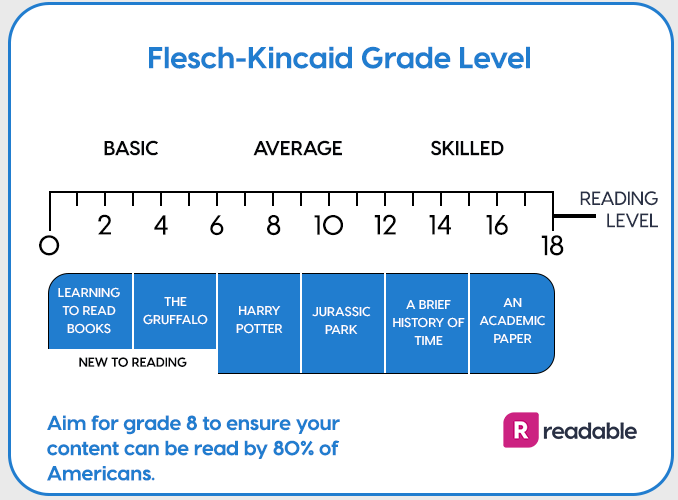
\includegraphics[width=\linewidth]{img/Screenshot_302.png}
	\caption{\autocite{Readable2021}}
\end{figure}

%---------- Methodologie ------------------------------------------------------
\section{Methodologie}%
\label{sec:methodologie}
Een \textit{mixed-methods} toont aan hoe toepassingen de inhoud van een wetenschappelijke paper geautomatiseerd kunnen vereenvoudigen, specifiek gericht op scholieren in de derde graad middelbaar. Het onderzoek houdt vijf grote fases in. De eerste fase is het proces van geautomatiseerde tekstvereenvoudiging beschrijven. Dit gebeurt via een grondige studie van vakliteratuur en wetenschappelijke teksten. Ook blogs van experten komen hier aan bod. Na het verwerven van de nodige inzichten wordt er een verklarende tekst opgesteld.

De tweede fase bestaat uit het analyseren van wetenschappelijke werken over de bewezen voordelen van tekstvereenvoudiging bij scholieren met dyslexie van het derde graad middelbaar onderwijs. Hiervoor zijn geringe thesissen beschikbaar, die zorgvuldigheid vragen tijdens interpretatie. De resulterende tekst bevat de voordelen samen met hun wetenschappelijke onderbouwing.

De derde fase is opnieuw een beschrijving. Hier worden de valkuilen bij taalverwerking met AI-software nagegaan. Deze fase van het onderzoek brengt mogelijke nadelen en tekortkomingen van AI-software bij tekstsimplificatie aan het licht. Dit gebeurt aan de hand van een technische uitleg.

De vierde fase omvat een toelichting over beschikbare AI toepassingen voor tekstvereenvoudiging. Aan de hand van een veldonderzoek op het internet en bij bedrijven wordt een longlist opgesteld van beschikbare toepassingen voor tekstvereenvoudiging in het onderwijs. Met een requirementsanalyse wordt er een shortlist opgesteld van software. De shortlist vormt de basis voor de ontwikkeling van een prototype voor geautomatiseerde en adaptieve tekstvereenvoudiging.

De vijfde en laatste fase van het onderzoek richt zich op het testen en beoordelen van de geselecteerde AI-toepassingen. In dit experiment zullen scholieren met dyslexie in het derde graad middelbaar onderwijs de shortlisted AI toepassingen en het prototype uitproberen. Het doel is om de effectiviteit en gebruikersvriendelijkheid van deze toepassingen te beoordelen. Na een grondige analyse wordt er met de resultaten van de testfase bepaalt of de toepassingen aan de vereisten voldoen om wetenschappelijke papers te vereenvoudigen voor scholieren in het middelbaar onderwijs.

%---------- Verwachte resultaten ----------------------------------------------
\section{Verwacht resultaat, conclusie}
\label{sec:verwachte_resultaten}

% exclameren dat de tools goed automatiseren, maar weinig tot geen keuze aanreiken

Er wordt verwacht dat de huidige softwareoplossingen voor tekstvereenvoudiging onvoldoende aansluiten bij de noden van scholieren met dyslexie in het derde graad middelbaar onderwijs. Het prototype is moeilijk af te stemmen op de specifieke noden van deze doelgroep. Er is nood aan aangepaste transformers om bevredigende resultaten te bereiken. Bovendien is er een gebrek aan Nederlandstalige word embeddings die de complexiteit van elk woord kunnen bijhouden en aan kant-en-klare modellen die de inhoud van wetenschappelijke papers kunnen vereenvoudigen. Word embeddings uit een Germaanse taal gebruiken, gevolgd door vertaling naar het Nederlands is wel een aanvaardbaar alternatief. 

%Er zijn te weinig kant-en-klare algoritmen en modellen beschikbaar om een pipeline voor tekstvereenvoudiging op te zetten, gericht op scholieren met dyslexie in het middelbaar onderwijs. 

